%\documentclass[../main.tex]{subfiles}

\begin{song}{title=\centering Slavíci z Madridu \\\normalsize Waldemar Matuška \vspace*{-0.3cm}}  %% sem se napíše jméno songu a autor
\moveright 4.5cm \vbox{      %Varianta č. 1  ---> Jeden sloupec zarovnaný na střed	

\sloka
^{Ami}Nebe je ^{E}modrý a zlatý, ^{Ami}bílá sluneční záře,

horko a ^{E}sváteční šaty, ^{Ami}vřava a zpocený tváře,

vím, co ^{E}se bude dít, býk už ^{Ami}se v ohradě vzpíná,

kdo chce, ^{E}ten může jít, já ^{Ami}si dám sklenici vína.

\refren
^{Dmi}Žízeň je ^{Ami}veliká, život mi utíká,

^{E}nechte mě ^{Ami}příjemně snít,

^{Dmi}ve stínu pod ^{Ami}fíky poslouchat slavíky

^{E}zpívat si s ^{Ami}nima a pít.

\sloka
Ženy jsou krásný a cudný, mnohá se ve mně zhlídla,

oči jako dvě studny, vlasy jak havraní křídla,

dobře vím, co znamená pád do nástrah dívčího klína,

někdo má pletky rád, já si dám sklenici vína.

\refren

\sloka
Nebe je modrý a zlatý, ženy krásný a cudný,

mantily, sváteční šaty, oči jako dvě studny,

zmoudřel jsem stranou od lidí, jsem jak ta zahrada stinná,

kdo chce, ať mi závidí, já si dám sklenici vína.

\refren

}
\setcounter{Slokočet}{0}

\end{song}
\begin{figure}[h]
\centering

\includegraphics[scale=1.5]{../Akordy/am}
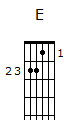
\includegraphics[scale=1.5]{../Akordy/e}
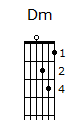
\includegraphics[scale=1.5]{../Akordy/dm}
\end{figure}

